\documentclass{standalone}
\usepackage{tikz}
\usetikzlibrary{patterns, positioning}


\begin{document}
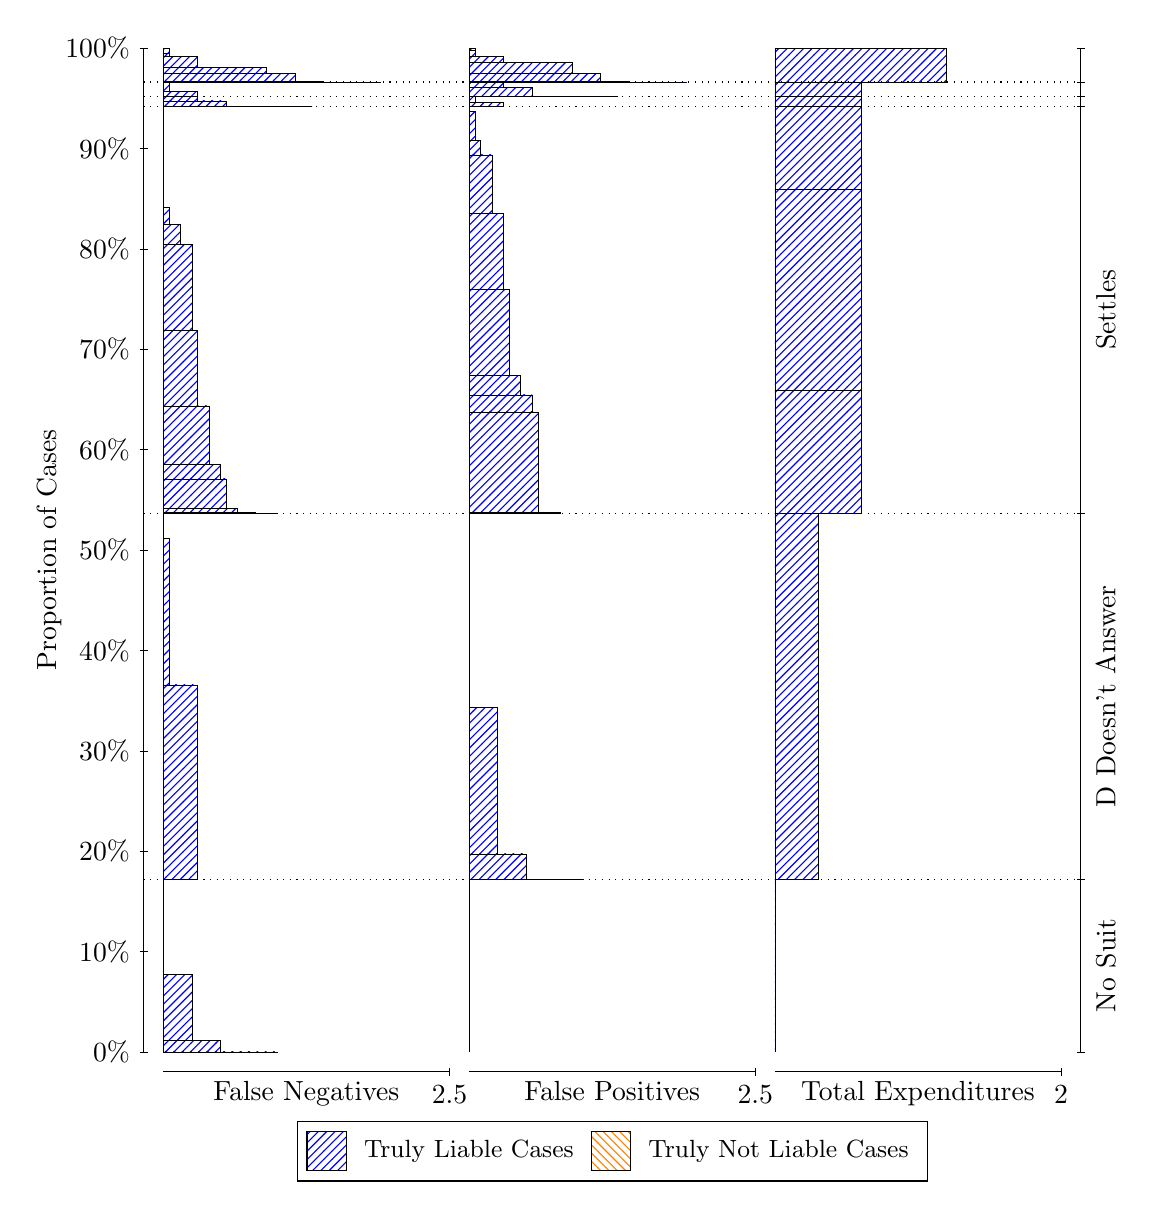
\begin{tikzpicture}
\draw[black, very thin] (1.5,1.75) -- (1.5,14.5);
\node[rotate=90, text=black, anchor=center] at (0.3, 8.125) {Proportion of Cases};
\draw[black, very thin] (1.45,1.75) -- (1.55,1.75);
\node[text=black, anchor=east] at (1.45, 1.75) {0\%};
\draw[black, very thin] (1.45,3.025) -- (1.55,3.025);
\node[text=black, anchor=east] at (1.45, 3.025) {10\%};
\draw[black, very thin] (1.45,4.3) -- (1.55,4.3);
\node[text=black, anchor=east] at (1.45, 4.3) {20\%};
\draw[black, very thin] (1.45,5.575) -- (1.55,5.575);
\node[text=black, anchor=east] at (1.45, 5.575) {30\%};
\draw[black, very thin] (1.45,6.85) -- (1.55,6.85);
\node[text=black, anchor=east] at (1.45, 6.85) {40\%};
\draw[black, very thin] (1.45,8.125) -- (1.55,8.125);
\node[text=black, anchor=east] at (1.45, 8.125) {50\%};
\draw[black, very thin] (1.45,9.4) -- (1.55,9.4);
\node[text=black, anchor=east] at (1.45, 9.4) {60\%};
\draw[black, very thin] (1.45,10.675) -- (1.55,10.675);
\node[text=black, anchor=east] at (1.45, 10.675) {70\%};
\draw[black, very thin] (1.45,11.95) -- (1.55,11.95);
\node[text=black, anchor=east] at (1.45, 11.95) {80\%};
\draw[black, very thin] (1.45,13.225) -- (1.55,13.225);
\node[text=black, anchor=east] at (1.45, 13.225) {90\%};
\draw[black, very thin] (1.45,14.5) -- (1.55,14.5);
\node[text=black, anchor=east] at (1.45, 14.5) {100\%};

\draw[black, very thin] (13.4,1.75) -- (13.4,14.5);
\draw[black, very thin] (13.35,1.75) -- (13.45,1.75);
\node[anchor=west] at (13.35, 1.75) {};
\draw[black, very thin] (13.35,3.9425) -- (13.45,3.9425);
\node[anchor=west] at (13.35, 3.9425) {};
\draw[black, very thin] (13.35,8.593) -- (13.45,8.593);
\node[anchor=west] at (13.35, 8.593) {};
\draw[black, very thin] (13.35,13.759) -- (13.45,13.759);
\node[anchor=west] at (13.35, 13.759) {};
\draw[black, very thin] (13.35,13.884) -- (13.45,13.884);
\node[anchor=west] at (13.35, 13.884) {};
\draw[black, very thin] (13.35,14.068) -- (13.45,14.068);
\node[anchor=west] at (13.35, 14.068) {};
\draw[black, very thin] (13.35,14.5) -- (13.45,14.5);
\node[anchor=west] at (13.35, 14.5) {};

\draw[black, very thin, pattern color=blue, pattern=north east lines] (1.75,1.75) rectangle (3.2033,1.75);
\draw[black, very thin, pattern color=blue, pattern=north east lines] (1.75,1.75) rectangle (2.84,1.7513);
\draw[black, very thin, pattern color=blue, pattern=north east lines] (1.75,1.7513) rectangle (2.4767,1.899);
\draw[black, very thin, pattern color=blue, pattern=north east lines] (1.75,1.899) rectangle (2.1133,2.7344);
\draw[black, very thin, pattern color=orange, pattern=north west lines] (1.75,2.7344) rectangle (1.75,2.7344);
\draw[black, very thin, pattern color=blue, pattern=north east lines] (1.75,2.7344) rectangle (1.75,3.9425);
\draw[black, very thin, pattern color=blue, pattern=north east lines] (1.75,3.9425) rectangle (2.186,6.4107);
\draw[black, very thin, pattern color=blue, pattern=north east lines] (1.75,6.4107) rectangle (1.8227,8.271);
\draw[black, very thin, pattern color=orange, pattern=north west lines] (1.75,8.271) rectangle (1.75,8.271);
\draw[black, very thin, pattern color=blue, pattern=north east lines] (1.75,8.271) rectangle (1.75,8.593);
\draw[black, very thin, pattern color=blue, pattern=north east lines] (1.75,8.593) rectangle (3.2033,8.593);
\draw[black, very thin, pattern color=blue, pattern=north east lines] (1.75,8.593) rectangle (3.058,8.5931);
\draw[black, very thin, pattern color=blue, pattern=north east lines] (1.75,8.5931) rectangle (2.9127,8.6035);
\draw[black, very thin, pattern color=blue, pattern=north east lines] (1.75,8.6035) rectangle (2.84,8.6043);
\draw[black, very thin, pattern color=blue, pattern=north east lines] (1.75,8.6043) rectangle (2.6947,8.6548);
\draw[black, very thin, pattern color=blue, pattern=north east lines] (1.75,8.6548) rectangle (2.5493,9.0281);
\draw[black, very thin, pattern color=blue, pattern=north east lines] (1.75,9.0281) rectangle (2.4767,9.2083);
\draw[black, very thin, pattern color=blue, pattern=north east lines] (1.75,9.2083) rectangle (2.3313,9.9562);
\draw[black, very thin, pattern color=blue, pattern=north east lines] (1.75,9.9562) rectangle (2.186,10.913);
\draw[black, very thin, pattern color=blue, pattern=north east lines] (1.75,10.913) rectangle (2.1133,12.005);
\draw[black, very thin, pattern color=blue, pattern=north east lines] (1.75,12.005) rectangle (1.968,12.257);
\draw[black, very thin, pattern color=blue, pattern=north east lines] (1.75,12.257) rectangle (1.8227,12.473);
\draw[black, very thin, pattern color=orange, pattern=north west lines] (1.75,12.473) rectangle (1.75,12.473);
\draw[black, very thin, pattern color=blue, pattern=north east lines] (1.75,12.473) rectangle (1.75,13.759);
\draw[black, very thin, pattern color=blue, pattern=north east lines] (1.75,13.759) rectangle (3.6393,13.759);
\draw[black, very thin, pattern color=blue, pattern=north east lines] (1.75,13.759) rectangle (3.276,13.759);
\draw[black, very thin, pattern color=blue, pattern=north east lines] (1.75,13.759) rectangle (2.9127,13.761);
\draw[black, very thin, pattern color=blue, pattern=north east lines] (1.75,13.761) rectangle (2.5493,13.83);
\draw[black, very thin, pattern color=blue, pattern=north east lines] (1.75,13.83) rectangle (2.186,13.884);
\draw[black, very thin, pattern color=orange, pattern=north west lines] (1.75,13.884) rectangle (1.75,13.884);
\draw[black, very thin, pattern color=blue, pattern=north east lines] (1.75,13.884) rectangle (2.186,13.952);
\draw[black, very thin, pattern color=blue, pattern=north east lines] (1.75,13.952) rectangle (1.8227,14.062);
\draw[black, very thin, pattern color=orange, pattern=north west lines] (1.75,14.062) rectangle (1.75,14.062);
\draw[black, very thin, pattern color=blue, pattern=north east lines] (1.75,14.062) rectangle (1.75,14.068);
\draw[black, very thin, pattern color=blue, pattern=north east lines] (1.75,14.068) rectangle (4.5113,14.068);
\draw[black, very thin, pattern color=blue, pattern=north east lines] (1.75,14.068) rectangle (4.148,14.068);
\draw[black, very thin, pattern color=blue, pattern=north east lines] (1.75,14.068) rectangle (3.7847,14.076);
\draw[black, very thin, pattern color=blue, pattern=north east lines] (1.75,14.076) rectangle (3.4213,14.174);
\draw[black, very thin, pattern color=blue, pattern=north east lines] (1.75,14.174) rectangle (3.276,14.174);
\draw[black, very thin, pattern color=blue, pattern=north east lines] (1.75,14.174) rectangle (3.058,14.251);
\draw[black, very thin, pattern color=blue, pattern=north east lines] (1.75,14.251) rectangle (2.9127,14.251);
\draw[black, very thin, pattern color=blue, pattern=north east lines] (1.75,14.251) rectangle (2.6947,14.251);
\draw[black, very thin, pattern color=blue, pattern=north east lines] (1.75,14.251) rectangle (2.5493,14.253);
\draw[black, very thin, pattern color=blue, pattern=north east lines] (1.75,14.253) rectangle (2.3313,14.253);
\draw[black, very thin, pattern color=blue, pattern=north east lines] (1.75,14.253) rectangle (2.186,14.255);
\draw[black, very thin, pattern color=blue, pattern=north east lines] (1.75,14.255) rectangle (2.186,14.394);
\draw[black, very thin, pattern color=blue, pattern=north east lines] (1.75,14.394) rectangle (1.8227,14.43);
\draw[black, very thin, pattern color=blue, pattern=north east lines] (1.75,14.43) rectangle (1.8227,14.494);
\draw[black, very thin, pattern color=orange, pattern=north west lines] (1.75,14.494) rectangle (1.75,14.494);
\draw[black, very thin, pattern color=blue, pattern=north east lines] (1.75,14.494) rectangle (1.75,14.5);
\draw[black, very thin, pattern color=orange, pattern=north west lines] (5.6333,1.75) rectangle (5.6333,1.75);
\draw[black, very thin, pattern color=blue, pattern=north east lines] (5.6333,1.75) rectangle (5.6333,3.9425);
\draw[black, very thin, pattern color=orange, pattern=north west lines] (5.6333,3.9425) rectangle (7.0867,3.9425);
\draw[black, very thin, pattern color=blue, pattern=north east lines] (5.6333,3.9425) rectangle (7.0867,3.9425);
\draw[black, very thin, pattern color=blue, pattern=north east lines] (5.6333,3.9425) rectangle (6.7233,3.9445);
\draw[black, very thin, pattern color=blue, pattern=north east lines] (5.6333,3.9445) rectangle (6.36,4.2645);
\draw[black, very thin, pattern color=blue, pattern=north east lines] (5.6333,4.2645) rectangle (5.9967,6.1248);
\draw[black, very thin, pattern color=blue, pattern=north east lines] (5.6333,6.1248) rectangle (5.6333,8.593);
\draw[black, very thin, pattern color=orange, pattern=north west lines] (5.6333,8.593) rectangle (6.796,8.593);
\draw[black, very thin, pattern color=blue, pattern=north east lines] (5.6333,8.593) rectangle (6.796,8.5984);
\draw[black, very thin, pattern color=orange, pattern=north west lines] (5.6333,8.5984) rectangle (6.6507,8.5984);
\draw[black, very thin, pattern color=blue, pattern=north east lines] (5.6333,8.5984) rectangle (6.6507,8.6035);
\draw[black, very thin, pattern color=orange, pattern=north west lines] (5.6333,8.6035) rectangle (6.5053,8.6035);
\draw[black, very thin, pattern color=blue, pattern=north east lines] (5.6333,8.6035) rectangle (6.5053,9.8792);
\draw[black, very thin, pattern color=blue, pattern=north east lines] (5.6333,9.8792) rectangle (6.4327,10.095);
\draw[black, very thin, pattern color=blue, pattern=north east lines] (5.6333,10.095) rectangle (6.2873,10.347);
\draw[black, very thin, pattern color=blue, pattern=north east lines] (5.6333,10.347) rectangle (6.142,11.439);
\draw[black, very thin, pattern color=blue, pattern=north east lines] (5.6333,11.439) rectangle (6.0693,12.396);
\draw[black, very thin, pattern color=blue, pattern=north east lines] (5.6333,12.396) rectangle (5.924,13.144);
\draw[black, very thin, pattern color=blue, pattern=north east lines] (5.6333,13.144) rectangle (5.7787,13.324);
\draw[black, very thin, pattern color=blue, pattern=north east lines] (5.6333,13.324) rectangle (5.706,13.697);
\draw[black, very thin, pattern color=blue, pattern=north east lines] (5.6333,13.697) rectangle (5.6333,13.759);
\draw[black, very thin, pattern color=orange, pattern=north west lines] (5.6333,13.759) rectangle (6.0693,13.759);
\draw[black, very thin, pattern color=blue, pattern=north east lines] (5.6333,13.759) rectangle (6.0693,13.813);
\draw[black, very thin, pattern color=blue, pattern=north east lines] (5.6333,13.813) rectangle (5.706,13.882);
\draw[black, very thin, pattern color=blue, pattern=north east lines] (5.6333,13.882) rectangle (5.6333,13.884);
\draw[black, very thin, pattern color=orange, pattern=north west lines] (5.6333,13.884) rectangle (7.5227,13.884);
\draw[black, very thin, pattern color=blue, pattern=north east lines] (5.6333,13.884) rectangle (7.5227,13.884);
\draw[black, very thin, pattern color=blue, pattern=north east lines] (5.6333,13.884) rectangle (7.1593,13.884);
\draw[black, very thin, pattern color=blue, pattern=north east lines] (5.6333,13.884) rectangle (6.796,13.89);
\draw[black, very thin, pattern color=blue, pattern=north east lines] (5.6333,13.89) rectangle (6.4327,14);
\draw[black, very thin, pattern color=blue, pattern=north east lines] (5.6333,14) rectangle (6.0693,14.068);
\draw[black, very thin, pattern color=orange, pattern=north west lines] (5.6333,14.068) rectangle (8.3947,14.068);
\draw[black, very thin, pattern color=blue, pattern=north east lines] (5.6333,14.068) rectangle (8.3947,14.068);
\draw[black, very thin, pattern color=orange, pattern=north west lines] (5.6333,14.068) rectangle (8.0313,14.068);
\draw[black, very thin, pattern color=blue, pattern=north east lines] (5.6333,14.068) rectangle (8.0313,14.068);
\draw[black, very thin, pattern color=orange, pattern=north west lines] (5.6333,14.068) rectangle (7.668,14.068);
\draw[black, very thin, pattern color=blue, pattern=north east lines] (5.6333,14.068) rectangle (7.668,14.074);
\draw[black, very thin, pattern color=orange, pattern=north west lines] (5.6333,14.074) rectangle (7.3047,14.074);
\draw[black, very thin, pattern color=blue, pattern=north east lines] (5.6333,14.074) rectangle (7.3047,14.174);
\draw[black, very thin, pattern color=blue, pattern=north east lines] (5.6333,14.174) rectangle (6.9413,14.315);
\draw[black, very thin, pattern color=orange, pattern=north west lines] (5.6333,14.315) rectangle (6.796,14.315);
\draw[black, very thin, pattern color=blue, pattern=north east lines] (5.6333,14.315) rectangle (6.796,14.315);
\draw[black, very thin, pattern color=blue, pattern=north east lines] (5.6333,14.315) rectangle (6.578,14.317);
\draw[black, very thin, pattern color=orange, pattern=north west lines] (5.6333,14.317) rectangle (6.4327,14.317);
\draw[black, very thin, pattern color=blue, pattern=north east lines] (5.6333,14.317) rectangle (6.4327,14.317);
\draw[black, very thin, pattern color=blue, pattern=north east lines] (5.6333,14.317) rectangle (6.2147,14.317);
\draw[black, very thin, pattern color=blue, pattern=north east lines] (5.6333,14.317) rectangle (6.0693,14.392);
\draw[black, very thin, pattern color=orange, pattern=north west lines] (5.6333,14.392) rectangle (6.0693,14.392);
\draw[black, very thin, pattern color=blue, pattern=north east lines] (5.6333,14.392) rectangle (6.0693,14.394);
\draw[black, very thin, pattern color=blue, pattern=north east lines] (5.6333,14.394) rectangle (5.8513,14.394);
\draw[black, very thin, pattern color=blue, pattern=north east lines] (5.6333,14.394) rectangle (5.706,14.472);
\draw[black, very thin, pattern color=blue, pattern=north east lines] (5.6333,14.472) rectangle (5.706,14.492);
\draw[black, very thin, pattern color=blue, pattern=north east lines] (5.6333,14.492) rectangle (5.6333,14.5);
\draw[black, very thin, pattern color=orange, pattern=north west lines] (9.5167,1.75) rectangle (9.5167,1.75);
\draw[black, very thin, pattern color=blue, pattern=north east lines] (9.5167,1.75) rectangle (9.5167,3.9425);
\draw[black, very thin, pattern color=orange, pattern=north west lines] (9.5167,3.9425) rectangle (10.062,3.9425);
\draw[black, very thin, pattern color=blue, pattern=north east lines] (9.5167,3.9425) rectangle (10.062,8.593);
\draw[black, very thin, pattern color=orange, pattern=north west lines] (9.5167,8.593) rectangle (10.607,8.593);
\draw[black, very thin, pattern color=blue, pattern=north east lines] (9.5167,8.593) rectangle (10.607,10.155);
\draw[black, very thin, pattern color=orange, pattern=north west lines] (9.5167,10.155) rectangle (10.607,10.155);
\draw[black, very thin, pattern color=blue, pattern=north east lines] (9.5167,10.155) rectangle (10.607,12.703);
\draw[black, very thin, pattern color=orange, pattern=north west lines] (9.5167,12.703) rectangle (10.607,12.703);
\draw[black, very thin, pattern color=blue, pattern=north east lines] (9.5167,12.703) rectangle (10.607,13.759);
\draw[black, very thin, pattern color=orange, pattern=north west lines] (9.5167,13.759) rectangle (10.607,13.759);
\draw[black, very thin, pattern color=blue, pattern=north east lines] (9.5167,13.759) rectangle (10.607,13.884);
\draw[black, very thin, pattern color=orange, pattern=north west lines] (9.5167,13.884) rectangle (10.607,13.884);
\draw[black, very thin, pattern color=blue, pattern=north east lines] (9.5167,13.884) rectangle (10.607,14.068);
\draw[black, very thin, pattern color=orange, pattern=north west lines] (9.5167,14.068) rectangle (11.697,14.068);
\draw[black, very thin, pattern color=blue, pattern=north east lines] (9.5167,14.068) rectangle (11.697,14.5);
\draw[black, dotted] (1.5,3.9425) -- (13.4,3.9425);
\draw[black, dotted] (1.5,8.593) -- (13.4,8.593);
\draw[black, dotted] (1.5,13.759) -- (13.4,13.759);
\draw[black, dotted] (1.5,13.884) -- (13.4,13.884);
\draw[black, dotted] (1.5,14.068) -- (13.4,14.068);
\draw[black, very thin] (1.75,1.5) -- (5.3833,1.5);
\node[text=black, anchor=north] at (3.5667, 1.5) {False Negatives};
\draw[black, very thin] (5.3833,1.45) -- (5.3833,1.55);
\node[text=black, anchor=north] at (5.3833, 1.45) {2.5};

\draw[black, very thin] (5.6333,1.5) -- (9.2667,1.5);
\node[text=black, anchor=north] at (7.45, 1.5) {False Positives};
\draw[black, very thin] (9.2667,1.45) -- (9.2667,1.55);
\node[text=black, anchor=north] at (9.2667, 1.45) {2.5};

\draw[black, very thin] (9.5167,1.5) -- (13.15,1.5);
\node[text=black, anchor=north] at (11.333, 1.5) {Total Expenditures};
\draw[black, very thin] (13.15,1.45) -- (13.15,1.55);
\node[text=black, anchor=north] at (13.15, 1.45) {2};

\node[text=black, centered, rotate=90] at (13.72, 2.8463) {No Suit};
\node[text=black, centered, rotate=90] at (13.72, 6.2678) {D Doesn't Answer};
\node[text=black, centered, rotate=90] at (13.72, 11.176) {Settles};




\draw (7.449999999999999,1.5) node[draw=none] (baseCoordinate) {};
\begin{scope}[align=center]
        \matrix[scale=0.5, draw=black, below=0.5cm of baseCoordinate, nodes={draw}, column sep=0.1cm]{
            \node[rectangle, draw, minimum width=0.5cm, minimum height=0.5cm, pattern color=blue, pattern=north east lines] {}; &
            \node[draw=none, font=\small, text=black] (B) {Truly Liable Cases}; &
            \node[rectangle, draw, minimum width=0.5cm, minimum height=0.5cm, pattern color=orange, pattern=north west lines] {}; &
            \node[draw=none, font=\small, text=black] (B) {Truly Not Liable Cases}; \\
            };
\end{scope}

\end{tikzpicture}
\end{document}